\scanpage{43}
que pour \unsure{tt|tout} segment $I$ de $S$, $I\subset S''$, il existe un plus grand segment de $S$ contenu dans $S'$ le contenant.

% slanted
\margin{introduire $\mathrm{Segm}_{\subset S'}(S\deleted{,\unsure{S'}})=\{I\subset S'\mid I\in\mathrm{Segm}(S)\}$}

Les éléments maximaux de $\mathrm{Segm}_{\subset S'}(S\deleted{,\unsure{S'}})$ sont appelés les \uline{segments \unsure{composants|comp.sants}} de la partie $S'$ de $S$.

% slanted
\margin{les élém. maximaux de $\mathrm{Segm}(S,S')$ i.e. les segments composants de $S'$, sont en corr. \unsure{1.1.} \unsure{resp.|pr.} \unsure{avec} les éléments \uline{minimaux} de l'ens des \deleted{\unsure{cl.|cl}} segments de $S$ qui \uline{contiennent} $S''$, par $I\mapsto S\setminus I$
\[
 \mathrm{Seg}_{\subset S'}(S)\overset{\unsure{\mathrm{antiiso.}}}{\simeq}\mathrm{Seg}_{\supset S''}(S)
\]}

Ils forment une partition de $S'$, d'où une relation d'équivalence dans $S'$.

En termes d'une réalisation top. de $(S,\{u,u^{-1}\})$ par un polygone top $(X,S)$, si $S''=S\setminus S'$, les \deleted{classes} segments de $S'$ sont en corr biunivoque avec les comp. conn. de $X\setminus S''$ qui rencontrent $S'$ -- ce sont les intersections de $S'$ avec ces comp. connexes.
\figure{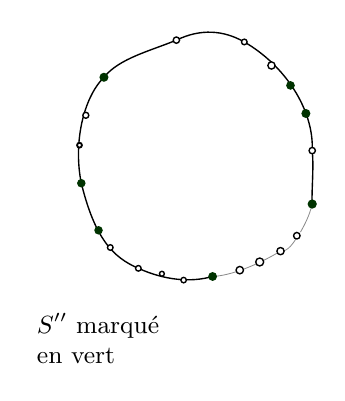
\begin{tikzpicture}[x=1.15cm,y=1.15cm,line width=.5pt]
\draw (-1.01,.97) .. controls (-.84,1.18) and (-.50,1.26) .. (-.21,1.38)
 .. controls (.06,1.51) and (.31,1.49) .. (.54,1.36)
 .. controls (.99,1.10) and (1.31,.61) .. (1.29,.16)
 .. controls (1.31,-.03) and (1.28,-.31) .. (1.29,-.43);
\draw[black!45,line width=.3pt] (1.29,-.43) .. controls (1.26,-.56) and (1.20,-.67) .. (1.16,-.74);
\draw[black!45,line width=.3pt] (1.13,-.78) .. controls (1.06,-.91) and (.99,-.96) .. (.94,-.95)
 .. controls (.69,-1.10) and (.40,-1.22) .. (.19,-1.23);
\draw (.19,-1.23) .. controls (-.06,-1.30) and (-.34,-1.27) .. (-.63,-1.14)
 .. controls (-.91,-1.02) and (-1.11,-.81) .. (-1.26,-.20)
 .. controls (-1.35,.24) and (-1.24,.74) .. (-1.01,.97);
\foreach \x/\y/\r in {-.21/1.38/.035,.54/1.36/.031,.84/1.10/.04,1.29/.16/.035,1.12/-.78/.036,.94/-.95/.04,.71/-1.07/.044,.49/-1.16/.041,-.13/-1.27/.03,-.37/-1.20/.027,-.63/-1.14/.031,-.94/-.91/.031,-1.21/.55/.033}
  \draw[fill=white] (\x,\y) circle[radius=\r];
\draw[line width=.65pt,fill=white] (-1.28,.22) circle[radius=.027];
\foreach \x/\y/\r in {-1.01/.97/.05,1.05/.88/.048,1.22/.57/.05,1.29/-.43/.051,.19/-1.23/.049,-1.07/-.72/.047,-1.26/-.20/.047}
  \fill[green!20!black] (\x,\y) circle[radius=\r];
\node[anchor=north west,align=left,font=\small] at (-1.86,-1.53) {$S''$ marqué\\en vert};
\end{tikzpicture}}

\uline{Proposition} Soient $A,B$ deux parties \deleted{disjointes non vides} de $S$, on suppose \deleted{$A$ et $B$}
\[
 A,B\ne\phi,S,\qquad A\cap B=\phi.
\]

Conditions équivalentes

% slanted
\margin{\uline{NB} On peut \inserted{prendre} pour $\bar A,\bar B$ les \inserted{\unsure{plus|des}} \deleted{\unsure{petits}} \deleted{\unsure{segments|sgmts}} composants}

a) $\exists$ segments $\bar A,\bar B$ de $S$, tels que $\bar A\supset A,\bar B\supset B$, $\bar A\cap\bar B=\phi$
% archive sheet number: 42
